\documentclass{scrbook}
\usepackage{siunitx}
\usepackage[version=4]{mhchem}
\usepackage{indentfirst}
\usepackage{tikz}
\usepackage{amsmath}
\usepackage{pgfplots}
\usepackage[backend=bibtex]{biblatex}
\usepackage{wrapfig}
\usetikzlibrary{positioning}
\addbibresource{Chemistry.bib}
\title{Chemistry Notes}
\subtitle{A level Chemistry}
\date{Last Updated \today{}}
\author{Dhruva Lokegaonkar}
\begin{document}
\maketitle
\tableofcontents

\chapter{Lattice Energy}

\section{What is Lattice Energy}

	The energy given out when ions of opposite charges come together to form a crystalline lattice is called the lattice energy, $\Delta H_{latt}^\ominus$.

	\[ \ce{Na+(g) + Cl-(g) ->  NaCl(s) \qquad \Delta H^\ominus_{latt} = \SI{-787}{ \kilo\joule\per\mole } }\]

	\begin{quote}
		Lattice energy is the enthalpy change when \SI{1}{\mole} of an ionic compound is formed from its gaseous ions under standard conditions.
	\end{quote}

	Lattice Energy is always negative. As the ion size increases, or as ionic charge increases, lattice energy becomes more exothermic.

\section{Other Enthalpies}

\subsection{Enthalpy Change of Atomisation}

	\begin{quote}
		The standard enthalpy change of atomisation, $\Delta H_{at}^\ominus$, is the enthalpy change when \SI{1}{\mole} of gaseous atoms is formed from it's elements under standard conditions.
	\end{quote}

	\[ \ce{ Li(s) -> Li(g) \qquad \Delta H^\ominus_{at} = \SI{161}{\kilo\joule\per\mole} } \]

	The Values of $\Delta H^\ominus_{at}$ are always positive.

\subsection{Electron Affinity}

	The energy change occurring when a gaseous non metal atom accepts one electron is called the electron affinity. The symbol is $\Delta H^\ominus_{ea}$

	\begin{quote}
		The first electron affinity, $\Delta H^\ominus_{ea1}$, is the enthalpy when \SI{1}{\mole} of electrons is added to \SI{1}{\mole} of gaseous atoms to form \SI{1}{\mole} of gaseous atoms 1- ions under standard conditions.
	\end{quote}

	\[ \ce{ Cl(g) + e- -> Cl-(g) \qquad \Delta H^\ominus_{ea1} = \SI{-348}{\kilo\joule\per\mole} } \]

	$\Delta H^\ominus_{ea1}$ is usually negative.

	\begin{quote}
		The second electron affinity, $\Delta H^\ominus_{ea2}$, is the enthalpy when \SI{1}{\mole} of electrons is added to \SI{1}{\mole} of gaseous 1- ions to form \SI{1}{\mole} of gaseous atoms 2- ions under standard conditions.
	\end{quote}

	\[ \ce{ O-(g) + e- -> O^2-(g) \qquad \Delta H^\ominus_{ea2} = \SI{798}{\kilo\joule\per\mole} } \]

	$\Delta H^\ominus_{ea2}$ and $\Delta H^\ominus_{ea3}$ are always positive

\section{Born-Haber Cycle}

	\begin{wrapfigure}{R}{0.3\linewidth}
	\centering
	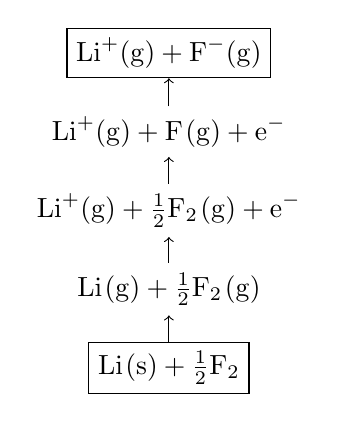
\begin{tikzpicture}[node distance=10mm]
		\node (a) [rectangle, draw] {$\ce{Li(s) + \frac{1}{2}F2}$};
		\node (b) [above of=a] {$\ce{Li(g) + \frac{1}{2}F2(g)}$};
		\node (c) [above of=b] {$\ce{Li+(g) + \frac{1}{2}F2(g) + e-}$};
		\node (d) [above of=c] {$\ce{Li+(g) + F(g) + e-}$};
		\node (e) [rectangle, draw, above of=d] {$\ce{Li+(g) + F-(g)}$};
		
		\draw[->] (a) -- (b);
		\draw[->] (b) -- (c);
		\draw[->] (c) -- (d);
		\draw[->] (d) -- (e);
	\end{tikzpicture}
	\caption{$\Delta H^\ominus_1$ in detail}
	\label{dh1}
	\end{wrapfigure}

	A Born-Haber cycle is a particular type of enthalpy cycle used to calculate lattice energy. Fig.\ref{bhc} shows a summary of the cycle. The $\Delta H^\ominus_1$ is the enthalpy involved in changing the elements from their standard states to their gaseous ionic states. Fig \ref{dh1} shows it in greater detail. $\Delta H^\ominus_1$ is the sum of each step converting from Lithium and Florine in standard states to the ionic states.  


	\begin{figure}[t]
	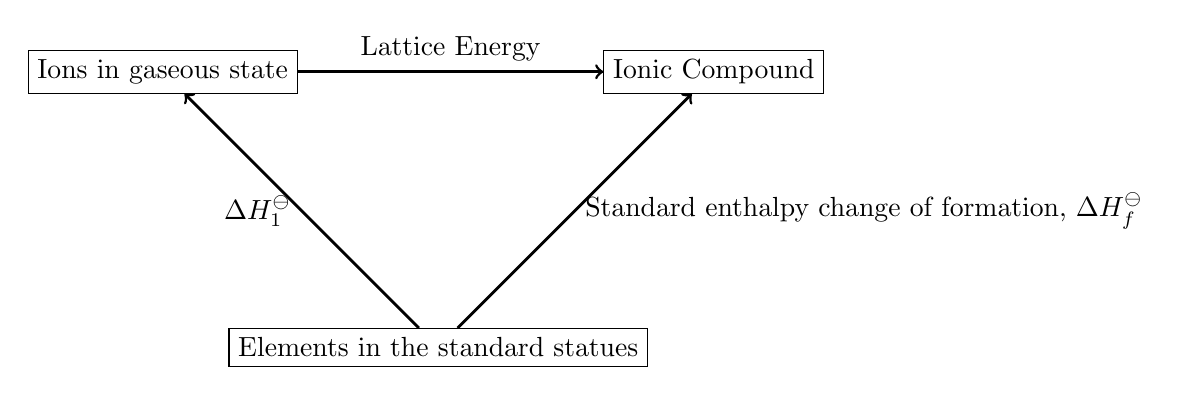
\begin{tikzpicture}[node distance=35mm]
		\node (ground) [rectangle, draw] {Elements in the standard statues};
		\node (ions) [rectangle, draw, above of=ground, left of=ground] {Ions in gaseous state};
		\node (comp) [rectangle, draw, above of=ground, right of=ground] {Ionic Compound};

		\draw[->, line width=1pt] (ground) -- node[left] {$\Delta H^\ominus_1$} (ions);	
		\draw[->, line width=1pt] (ground) to node[right] {Standard enthalpy change of formation, $\Delta H^\ominus_f$} (comp);
		\draw[->, line width=1pt] (ions) to node[auto] {Lattice Energy} (comp);

	\end{tikzpicture}
	\caption{Born-Haber Cycle}
	\label{bhc}
	\end{figure}

\section{Ion Polarisation}

	Sometimes the positive change on the cation in a ionic lattice may attract the electrons on the cation causing a distortion in the electron cloud. The anion is more likely to be polarised if:

	\begin{itemize}
		\item
			The cation is small or the anion is large.
		\item
			The cation has a large positive charge or the anion has a large negative charge.
	\end{itemize}

	\begin{figure}[h]
		\centering
		\caption{Ion Polarisation and distortion \cite{hrofchem}}
		\label{polar}
		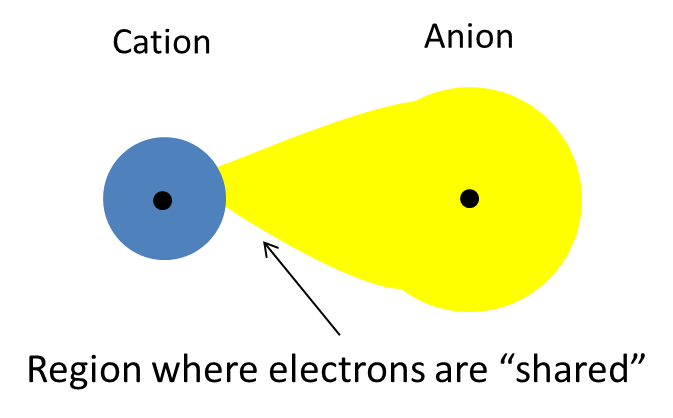
\includegraphics[width=0.5\linewidth]{assets/polar.png}
	\end{figure}

\section{Enthalpy changes in solution}

	\begin{quote}
		The enthalpy change of solution, $\Delta H^\ominus_{sol}$, is the energy absorbed or released when \SI{1}{\mole} of ionic solid dissolves in sufficient water to form a very dilute solution
	\end{quote}

	\[ \ce{MgCl(s) + aq -> Mg^{2+}(aq) + 2Cl-(aq) } \qquad \Delta H^\ominus_{sol} = \SI{-55}{\kilo\joule\per\mole} \]

	The value of $\Delta H^\ominus_{sol}$ is much less than $\Delta H^\ominus_{latt}$ because a lot of energy to overcome to lattice energy comes from the strong attraction between the ions and the molecules of water. This is called the enthalpy change of hydration.

	\begin{quote}
		The enthalpy change of hydration, $\Delta H^\ominus_{hyd}$, is the enthalpy change when \SI{1}{\mole} of a specified gaseous gaseous ion dissolves in sufficient water to form a very dilute solution
	\end{quote}

	\begin{figure}[h]
	\centering
	\caption{Hess diagram for $\Delta H^\ominus_{hyd}$}
	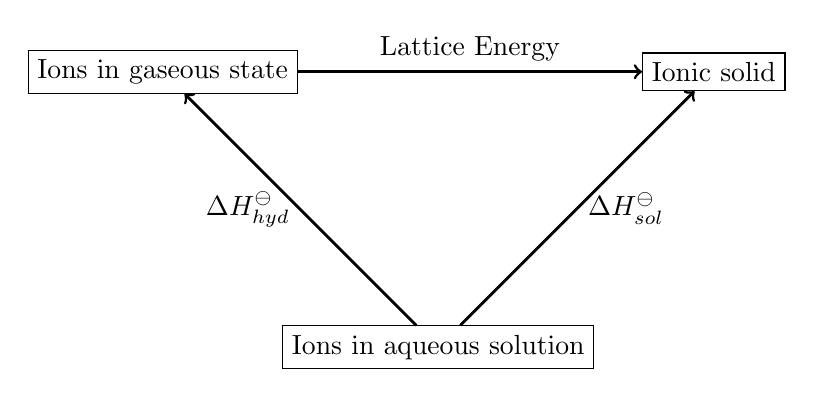
\begin{tikzpicture}[node distance=35mm]
                \node (ground) [rectangle, draw] {Ions in aqueous solution};
                \node (ions) [rectangle, draw, above of=ground, left of=ground] {Ions in gaseous state};
                \node (comp) [rectangle, draw, above of=ground, right of=ground] {Ionic solid};

			\draw[->, line width=1pt] (ground) -- node[left] {$\Delta H^\ominus_{hyd}$} (ions);
			\draw[->, line width=1pt] (ground) to node[right] {$\Delta H^\ominus_{sol}$} (comp);
                \draw[->, line width=1pt] (ions) to node[auto] {Lattice Energy} (comp);
	\end{tikzpicture}
	\end{figure}

	The decrease in solubility of Group 2 sulphates can be explained in terms of the relative values of the enthalpy change of hydration and the corresponding lattice energies.

\chapter{Electrochemistry}

\section{Electrolysis}

\subsection{Electrolytic cells}

	\begin{quote}
		Electrolysis is the decomposition of a compound by an electric current
	\end{quote}

	Electrolysis is carried out in an electrolysis cell. The electrolyte is the compound that is decomposed. The electrodes are rods which conduct electricity. Anodes are positive electrodes and Cathodes are negative. The power supply is always a Direct Current.

\subsection{Redox reactions}

	Electrolysis is a redox reaction. During electrolysis positive ions move to the cathode and gain electrons, where as the negative ions move to the anode and lose electrons. The electrolysis of Zinc Chloride can be summarised by the following reactions:

	\begin{align*}
		\text{Cathode :} && \ce{Zn^{2+} + 2e- &-> Zn} \\
		\text{Anode :} && \ce{2Cl- &-> Cl2 + 2e-} \\
		\text{Overall :} && \ce{ZnCl2 &-> Zn + Cl2}
	\end{align*}

\section{Quantitative electrolysis}

	The mass of the substance deposited is directly proportional to the charge that flows through the electrolyte. The charge of \SI{1}{\mole} of electrons is said to be 1 Faraday. It's value is equal to \SI{96500}{\coulomb\per\mole}. This can be used to calculate the mass of the deposited substance. For example, in the following equations, \ce{Cu^{2+}} required \SI{2}{\mole} of electrons to produce \SI{1}{\mole} of \ce{Cu} atoms.

	\[ \ce{Cu^{2+} +2e- -> Cu} \]

	This means it needs 2 Faraday of electricity to produce \SI{1}{\mole} of \ce{Cu}. If a current of $x$ amperes went through it for $t$ seconds, a charge of $xt$ went through the cell. The number of Faraday that passed through the electrolyte is:

	\[ F = \frac{xt}{96500} \]

	The number of moles of \ce{Cu} is half that value. The mass can be calculated by multiplying the molar mass of \ce{Cu} to the number of moles of \ce{Cu}

\section{Electrode Potentials}

\subsection{Metal/Metal ion system}

	When a metal is placed into a solution of it's ions, an electric potential is established between the metal and the metal ion solution. This potential is not measurable but the difference between the metal/metal ion system and another system can be measured.

\subsection{Electrode potentials and redox reactions}

	Electrode potential values give us an indication of how easy it is to reduce a substance. The more positive the electrode potential is, the easier is it to reduce it's ions.

\subsection{Standard electrode potential}

	The voltage of an electrochemical cell is affected by concentration, temperature and pressure. Hence, when comparing electrode potentials, standard conditions are used. There are:

	\begin{itemize}
		\item
			Concentration of ions at \SI{1.00}{\mole\per\deci\metre\cubed}
		\item
			Temperature at \SI{25}{\celsius} (\SI{298}{\kelvin})
		\item
			Gasses at \SI{1}{atm} (\SI{101}{\kilo\pascal})
		\item
			The value of the electrode potential is measured against the standard hydrogen electrode.
	\end{itemize}

	\begin{quote}
		The electrode potential, $H^\ominus$, for a half-cell is the voltage measured under standard conditions with a standard hydrogen electrode as the other half-cell.
	\end{quote}

\section{Using $E^\ominus$ values}

\subsection{Using $E^\ominus$ values to predict cell voltages}

	$E^\ominus$ values can be used to calculate the voltage of an electrochemical cell made up of two half-cells. It is the difference between the $E^\ominus$ values of the two cells. Consider a cell with a \ce{Ag/Ag+} half cell at the cathode and a \ce{Zn/Zn+} cell at the anode.

	\begin{align*}
		\ce{ Ag+ (aq) + e- &<=> Ag(s) } && &E^\ominus &= \SI[explicit-sign=+]{0.80}{\volt} \\
		\ce{ Zn^{2+} (aq) +2e- &<=> Zn (s) } && &E^\ominus &= \SI[explicit-sign=+]{-0.76}{\volt}
	\end{align*}

	The voltage of this cell is \SI{1.56}{\volt}

\subsection{$E^\ominus$ values can help deduce the direction of electron flow}

	Looking at the previous equations again, we can see that \ce{Zn^{2+}} ions are more difficult to reduce than \ce{Ag+} ions. So, the \ce{Zn} metal will lose electrons to the \ce{Ag+/Ag} half-cell, and the \ce{Ag=} ions will accept electrons from the \ce{Zn^{2+}/Zn} half-cell. Electrons will flow from the \ce{Zn^{2+}/Zn} half-cell to the \ce{Ag+/Ag} half cell in the circuit.

\subsection{Using $E^\ominus$ values to predict of a reaction will occur}

	The $E^\ominus$ values tell us how good of a reducing agent or oxidising agent a chemical is.

	\begin{itemize}
		\item
			The more positive the value of $E^\ominus$, the greater the tendency for the half-equation to proceed in the forward direction, the better oxidising agent it is.
		\item
			The less positive the value of $E^\ominus$, the greater the tendency for the half-equation to proceed in the backward direction, the better reducing agent it is.
	\end{itemize}

	A reaction occurs in a direction such that the stronger oxidising agent oxidises the stronger reducing agent. For example, we can answer the question whether Chlorine will oxidise \ce{Fe^{2+}} ions to \ce{Fe^{3+}} ions, by looking at their half-equations.

	\begin{align*}
		\ce{ 1/2Cl2 (g) + e- &<=> Cl- (aq)} && &E^\ominus &= \SI[explicit-sign=+]{1.36}{\volt} \\
		\ce{ Fe^{3+} (aq) + e- &<=> Fe^{2+} (aq) } && &E^\ominus &= \SI[explicit-sign=+]{0.77}{\volt}
	\end{align*}

	We can see that \ce{Cl2} is a better oxidising agent that \ce{Fe^{2+}} and \ce{Cl2} oxidising \ce{Fe^{2+}} to \ce{Fe^{3+}} is feasible.

	\[ \ce{1/2Cl2 (g) + Fe^{2+} (aq) -> Cl- (aq) + Fe^{3+} (aq) } \]'=

\section{Non standard Electrode Potentials}

	The effect of concentration and temperature on the value of $E_{\text{cell}}$ can be deduced by using the Nerst equation. For a given electrode, the electrode potential, $E$, is given by,

	\[ E = E^\ominus + \frac{RT}{zF}\ln{\frac{\text{[oxidised form]}}{\text{[reduced form]}}} \]

	\begin{align*}
		\text{Where } 
		& E^\ominus \text{ is the standard electrode potential} \\
		& R \text{ is the gas constant \SI{8.314}{\joule\per\kelvin\per\mole}} \\
		& T \text{ is the temperature in Kelvin} \\
		& z \text{ is the number of electrons transferred in the reaction} \\
		& F \text{ is the value of the Faraday constant, \SI{96500}{\coulomb\per\mole}}
	\end{align*}

\section{Cells and Batteries}

	At this point im bored as heck. Summarise the following sub topics in the book and send me, I'll add it here:

	\begin{itemize}
		\item
			Rechargable Cells
		\item
			Solid state Cells
		\item
			Hydrogen-oxygen fuel Cells
	\end{itemize}

	The rest is useless.

\chapter{Equilibria}

\section{Equilibrium constant and pH}

	The equilibrium constant is:

	\[ K_c = \frac{[\text{[Products}]}{[\text{Reactants}]} \]

	Water also exists in an equilibrium where it acts a both an acid and a base.

	
	\[ \ce{H20 (l) -> H+ (aq) + OH- (aq) } \]

	Where. $K_c = \frac{\ce{[H+ (aq)]}\ce{[OH- (aq)]}}{\ce{[H2O (l)]}}$. Since the concentration of water is constant, and the concentrations of Hydrogen and Hydroxide ions is equal, we can create a new equation:

	\[ K_w = \ce{[H+]}^2 \]

	$K_w$ is called the ionic product of water.

	\begin{quote}
		pH is defined as the negative logarithm to the base 10 of hydrogen ion concentration
	\end{quote}

	\[ \text{pH} = -\log_{10}\ce{[H+]} \]

	The equilibrium constant for the dissociation equation of a acid is called the acid dissociation constant, $K_a$

	\[ K_a = \frac{\ce{[H]}\ce{[A]}}{\ce{[HA]}} \qquad and \qquad \text{p}K_a = -\log_{10}K_a \]

\section{Buffer Solution}

	A buffer solution is a solution whose pH does not change significantly when small amounts of acid or base are added. They are usually a solution of a weak acid and one of its salts. For a buffer solution, 

	\begin{align*}
		\ce{[H+]} &= K_a \times \frac{\text{[acid]}}{\text{[salt]}} \\
		\text{pH} &= \text{p}K_a + \log_{10}\left(\frac{\text{[salt]}}{\text{[acid]}}\right)
	\end{align*}

\section{Solubility product and Common ion effect}

	\begin{quote}
		Solubility product is the product of the concentrations of each ion in a saturated solution of a sparing soluble salt at \SI{298}{\kelvin}, raised to the power of their relative concentrations.
	\end{quote}

	For the example equation:

	\[ \ce{A_bC_q <=> aC^{y+} + bA^{x-}} \]

	The solubility constant, $K_{sp}$, is:

	\[ K_{sp} = \ce{[C^{y+}]}^a\ce{[A^{x-}]}^b \]

	\begin{quote}
		The common ion effect is the reduction in solubility of a dissolved salt achieved by adding a solution of a compound which has an ion in common with the dissolved salt.This often results in precipitation.
	\end{quote}

\printbibliography{}
\end{document}
